\section{Analysis of second required behavior: Configuration adaptive vessel platform control}
\label{analysisConfigAdaptation}

\subsection{Problem Description}
We have a team of $n$ modules connected into a platform. $n$ can vary through time as modules connect or disconnect. 
There exists an expression of the state of the platform expressed similar to single vessels as:

\begin{equation}
\eta_p = \begin{bmatrix} \textbf{p}^{n}_{p} \\[8pt]  \Theta_{np} \end{bmatrix} = \begin{bmatrix} x^{n}_{p} \\[8pt]  y^{n}_{p} \\[8pt] \Psi^n_p \end{bmatrix}
\end{equation}

\begin{equation}
\nu_p = \begin{bmatrix} \textbf{v}^{p}_{p/n} \\[8pt]  \omega^{p}_{p/n} \end{bmatrix} = \begin{bmatrix} u\\v\\r \end{bmatrix}
\end{equation}

Where $\eta_p$ and $\nu_p$ describe generalized positions and velocities of the platform coordinate system origin.  If the platform connections can be assumed rigid, a platform fixed coordinate system can be made that defines platform state in the above mentioned $\eta_p$ and $\nu_p$. Other definitions of platform state can be fixed to a single vessel, which does not assume rigid connections, or by coinciding the platform origin with its estimated overall centre of mass. Figure \ref{fig:bartned_platform_frame} illustrates an example of a platform coordinate system fixed to the vessels, where in this definition the origin of the platform is even a little outside the body of the platform. 

\begin{figure}[h!]
	\centering
	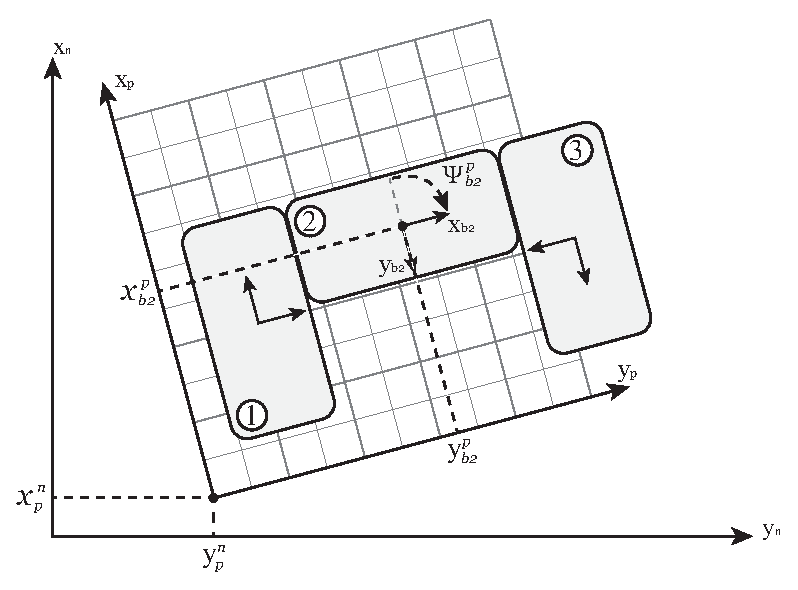
\includegraphics[width=0.8\textwidth]{ned_platform_frame}
	\caption{A platform consisting of three modules. Expression of pose of vessel 2 in the platform coordinate system ($ \{p\}$) is illustrated, as well as position of the platform frame origin in global ($ \{n\}$) frame. This example shows the origin of the platform coordinate system outside of the physical body of the platform, but this placement can be chosen elsewhere at the convenience of the designer.}
	\label{fig:bartned_platform_frame}
\end{figure}

Each module $m_i$ has $r_i = 0,1,2,...$ actuators that are able to impose forces on that module to move it, such as propellers. The amount of actuators that modules have may not be equal for all vessels. This may be unequal by design (as in a heterogenous fleet) , or as a response to a noticed malfunctioning thruster. The total amount of actuators is the summation of the actuators of all vessels.

\begin{equation} 
r =\sum_{i=1}^{n} r_i
\end{equation}

Actuators are bound to various constraints such as direction and maximum force output. Acuators that make forces between vessels to connect them could be described as actuators as well, which can be benificial if connections are not considered rigid. Actuators have dynamics of their own, meaning that they often do not respond instantaneous. However, modelling the dynamics of actuators can  overcomplicate a total system model. If a model is to be kept simple, one can assume that execution of actuator reference is done sufficiently accurate and timely. It is a good idea to reflect if this assumption is reasonable by evaluating the performance of used actuators to accurately follow control inputs, and judge whether inacurracy or delay will significantly affect overall system behavior. 

\subsection{Motion control systems}
Waterborn vehicle dynamics can be described according to \citet{fossen2011handbook}, where the author shows that translational motion of a vessel about CO satisfies

\begin{equation}
m [ \dot{\textbf{v}}_{b/n}^{b} + \dot{\omega}_{b/n}^{b}  \times \textbf{r}_g^b     + \omega_{b/n}^{b}  \times  \textbf{v}_{b/n}^{b} +  \omega_{b/n}^{b}  \times ( \omega_{b/n}^{b}  \times \textbf{r}_g^b   ) ] = \textbf{f}_b^b
\label{eq:fossen2011TranslationalMotionAboutCO-eqnumber-3-33}
\end{equation}

and that rotational motion of a vessel about CO satisfies

\begin{equation} 
\textbf{I}_b  \dot{\omega}_{b/n}^{b} + \omega_{b/n}^{b}  \times \textbf{I}_b \omega_{b/n}^{b}  + m \textbf{r}_g^b \times  ( \dot{\textbf{v}}_{b/n}^{b} +   	\omega_{b/n}^{b} 	 \times	\textbf{v}_{b/n}^{b}	) = \textbf{m}_b^b 
\label{eq:fossen2011RotationalMotionAboutCO-eqnumber-3-40} 
\end{equation}

where components in equation \ref{eq:fossen2011TranslationalMotionAboutCO-eqnumber-3-33} and \ref{eq:fossen2011RotationalMotionAboutCO-eqnumber-3-40} are defined as

\begin{table}[H]
	\centering
	\begin{tabular}{llll}
		$\boldmath{f}^{b}_{b} $ 	   	& = & $[X,Y,Z]^\top$ 		&	- Force with line of action through point $o_b$ expressed in coordinate system $\{b\}$ \\[5pt]
		$\boldmath{m}^{b}_{b} $   		& = & $[K,M,N]^\top$ 		&	- Moment about point $o_b$ expressed in coordinate system $\{b\}$ \\[5pt]
		$ \textbf{v}^{b}_{b/n}$   		& = & $[u,v,w]^\top$ 		&	- Linear velocity of point $o_b$ with respect to $o_n$ expressed in coordinate system $\{b\}$ \\[5pt]
		$ \omega^{b}_{b/n}$   			& = & $[p,q,r]^\top$ 		&	- Angular velocity of $\{b\}$ with respect to $\{n\}$ expressed in coordinate system $\{b\}$  \\[5pt]
		$\textbf{r}^{b}_{g} $ 			& = & $[x_g,y_g,z_g]^\top$ 	&	- Position of centre of gravity expressed in coordinate system $\{b\}$ 
	\end{tabular}
\end{table}

\citet{fossen1994guidance} expresses equation \ref{eq:fossen2011TranslationalMotionAboutCO-eqnumber-3-33} and \ref{eq:fossen2011RotationalMotionAboutCO-eqnumber-3-40} vectorial form
\begin{equation}
\textbf{M}_{RB} \dot{\nu} + \textbf{C}_{RB}(\nu)\nu  = \tau_{RB}
\label{eq:fossen1994RigidBodyKinetics1}
\end{equation}

where $ \textbf{M}_{RB} $ is the rigid body inertia matrix, $\textbf{C}_{RB}$ is a matrix of rigid-body Coriolis and centripetal forces due to the rotation of $\{b\}$ about the inertial frame $\{n\}$, $\nu$ is a vector with generalized velocities expressed in $\{b\}$ and $\tau_{RB}$ is a vector with generalized forces expressed in $\{b\}$. 

Dampening forces can be modelled linear with constant D matrix as 
\begin{equation}
\textbf{M}_{RB} \dot{\nu} + \textbf{C}_{RB}(\nu)\nu  + \textbf{D}\nu = \tau
\label{eq:fossen1994RigidBodyKineticsinclDampeningLinear}
\end{equation}


Or nonlinear as: 
\begin{equation}
\textbf{M}_{RB} \dot{\nu} + \textbf{C}_{RB}(\nu)\nu  + \textbf{D}(\nu)\nu = \tau
\label{eq:fossen1994RigidBodyKineticsinclDampeningNonLinear}
\end{equation}
Which can both be estimated by model identification experiments. Whether linear or nonlinear dampening models are suitable depends on the accuracy of tests and reasonabe operating range. It is common to model some hydrodynamic forces as constant additive accelleration coefficients. \citet{humphreys1978prediction} states that the forces and moments represented by the acceleration hydrodynamic coefficients can, to a very great extent, be modeled as potential flow phenomena, yielding 

\begin{equation}
\textbf{M} \dot{\nu} + \textbf{C}(\nu)\nu  + \textbf{D}(\nu)\nu = \tau{}
\label{eq:fossen1994RigidBodyKineticsinclAddedMass}
\end{equation}

where
\begin{equation}
\textbf{M} = \textbf{M}_{RB} + \textbf{M}_{A}
\end{equation}
Where $ \textbf{M}_{RB} $ represents inertia of the rigid module and $\textbf{M}_{A}$ represents hydrodynamic added mass. Similarly
\begin{equation}
\textbf{C}(\nu)\nu = \textbf{C}_{RB}(\nu)\nu + \textbf{C}_{A}(\nu)\nu
\end{equation}
Where $ \textbf{C}_{RB}(\nu)\nu $ and $\textbf{C}_{A}(\nu)\nu$ represent coriolis and centripetal forces of the rigid body and hydrodynamic added mass. 

Control forces of all actuators (of all modules) can be described in a vector format as:
\begin{equation}
\textbf{f} = [F_{1},F_{2},F_{3}, ... F_{r}]^\top
\end{equation}
Where $F_i$ is the control force generated by actuator $r_i$. 
If the relation between control input and resulting force can be assumed linear, the control forces can be expressed as:

\begin{equation}
\textbf{f} = \textbf{K} * \textbf{u}
\end{equation}

Where $\textbf{u}$ is a vector of control inputs and $\textbf{K}$ is a diagonal force coefficient matrix (see \citet{fossen2011handbook})

Control forces applied across the body can be expressed in total control forces:
\begin{equation}
\tau = \textbf{T}(\alpha)\textbf{f}
\end{equation}
Where $ \textbf{T}(\alpha) \in \mathbb{R}^{n\times r}$ is the thrust configuration matrix, dependent on angles $ \alpha = [\alpha_1,... \alpha_p]^\top \in \mathbb{R}^{p}$ of p rotatable thrusters. \citet{fossen2011handbook} shows how the use of angles of rotatable thrusters can be avoided in the above expression by decoupling the force of a rotatable thruster in two separate forces (generaly decoupled in x and y for surface vessels). Decoupling x and y components of a rotating thruster can simplify math challenges, but does require to take into account physical constraints of absolute maximum thrust of the actuator. 



The team of connected modules has a single, dynamic, multi-robot task, namely the control of actuators to satisfy a time varying platform state. What a satisfactory state actually is depends on the designer, but this is usually defined as a reference state, such as desired positions, and/or velocities.  Utilizing the concept of a reference state in a multi-robot collaborative system means that the controlling entity of a module or platform needs means to aquire the control objective. Various design options are possible to have a set of robots collaborating towards  achieving a single goal. The control objective can be created by various entities.
\begin{itemize}
	\item The robot can generate its own control objective, sensing the environment and following a decision protocol. 
	\item The control objective can be generated by another entity, such as another robot or an operator. This would require means of communication. 
\end{itemize}

\citet{parasuraman2000model} describes an approach on dividing a control problem in four stages with similarities to human decision making. This approach is general and intended to be applicable to a wide spectrum of robot systems, as shown in figure \ref{fig:parasuraman2000model-foursteps}, yet can be applied to a multi-robot system as well. The amount of agents in the multi robot system that collaboratively perform functionality of one of the stages can vary. Some tasks can be done by a single agent, while other tasks can be achieved with multiple. For example; sensing fleet state can be done by a single centralized agent, sending sensor data to on board decision makers, or each vessel can have its own means of sensing its surroundings. 
%\colorbox{yellow}{\parbox{12cm}{This is a very }}\\
%"The first stage refers to the acquisition and registration of multiple sources of information. This stage includes the positioning and orienting of sensory receptors, sensory processing, initial pre-processing of data prior to full perception, and selective attention. The second stage involves conscious perception, and manipulation of processed and retrieved information in working memory [13]. This stage also includes cognitive operations such as rehearsal, integration and inference, but these operations occur prior to the point of decision. The third stage is where decisions are reached based on such cognitive processing. The fourth and final stage involves the implementation of a response or action consistent with the decision choice." \cite{parasuraman2000model}

A collaborative multi vessel control system can thus have its tasks distributed across agents in many ways. To control $n$ vessels where each vessel is equipped with $r_i$ actuators, the following system components can be identified for a certain design divided as shown in \citet{parasuraman2000model}
\begin{itemize}
	\item i agents that aquire information about the state, or called sensing.
	\item j agents that interpret sensed information, converting it into concepts, such as a state estimate. 
	\item k agents that formulate sets of control options
	\item l agents that decide a control option from the set
\end{itemize}

\begin{figure}[H]
	\centering
	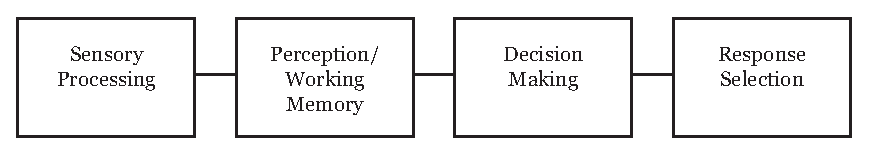
\includegraphics[width=0.8\textwidth]{parasuraman2000model-foursteps}
	\caption{Four-stage model of human information processing. \cite{parasuraman2000model}}
	\label{fig:parasuraman2000model-foursteps}
\end{figure}

Classic marine control theory pertains only a single ship. A common division of the overall control system into subsystems is according to the Guidance, Navigation and Control (GNC) scheme \cite{fossen2011handbook}. The navigation system uses sensors and an observer to generate a state estimate. The guidance system performs task planning and continuously generates a control objective or reference. This is used by the (motion) control system to coordinate responses of available actuators, such that the vessel response follows the reference. 

\subsection{Multi-robot Cooperation}
Various challenges in cooperative multi robot systems are systematically described in existing literature. A section of relevant terms and concepts will be discussed to adress the problem of this section. 

For a multi-robot system, the division of tasks to a set of robots is referred to as "task allocation" \citet{lerman2006analysis}. This is extended to "dynamic task allocation" if the assignment of tasks to robots needs to be adjusted continuously due to changes in task environment and system response. 
\citet{lerman2006analysis} describes a "distributed multi-robot system" as a MRS that does not have a central coordinator. Distribution and centralization of control structure both have their benefits and disadvantages. Decisions in distributed control systems need to be made with incomplete information, while a centralized decision making agent has the potential to use all available data. Centralized control structures have, however, a single point of failure and can encounter scaling issues. 

As multiple robots collaboratively seek to perform the common task of platform motion control, there are varying approaches to allocating control efforts with similar results, as a vessel platforms actuators are likely far more numerous than the (debatably consistent) degrees of freedom. \citet{fossen2011handbook} shows how a vessel motion control block is commonly divided into a dedicated subsystem that generates 'control efforts', and a block that allocates the desired control effort, by dividing it over the available actuators, schematically shown in figure \ref{fig:fossenControlAllocationPNG}. This approach is also used for the configuration adaptive vessel platform controller in \citet{park2019coordinated}, while therein control allocation is referred to as "coordination" and generation of control efforts is referred to as "robust control". 

 \begin{figure}[h!]
 	\centering
 	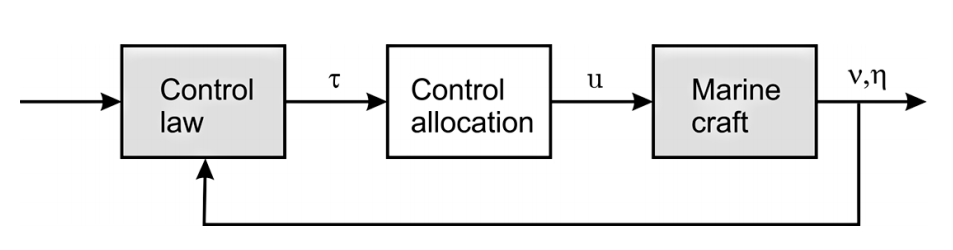
\includegraphics[width=0.6\textwidth]{fossen2011handbookControlAllocation}
 	\caption{Block diagram showing the control-allocation-block in a vessel motion control system. \cite{fossen2011handbook}.}
 	\label{fig:fossenControlAllocationPNG}
 \end{figure}
 
To use this methodology for control of vessel platform motion, the state estimation would need to pertain platform state, and not that of an individual vessel. This is generally positions $\eta_p$ and possibly velocities $\nu_p$, which are to be controlled to a desired state. Which parts of the state are to be controlled depends on the approach and complexity of the control system. Dynamic positioning, for instance, controls pose ($\eta = [x,y,\Psi]$) but not directly velocities ($\nu = [u,v,r]$).

\citet{park2019coordinated} utilizes a centralized control approach to generate control efforts that need to be applied on the platform, while their approach assumes rigid connections. Control effort generation was achieved by means of a PI controller. Control decisions are made centralized on one vessel that is elected as coordinator, which divides the control effort over platform modules. A schematic of the control loop of \citet{park2019coordinated} is  shown in figure \ref{fig:park2019coordinatedSontrolScheme}, showing various elements that could be sensibly interpreted with both the four stage model of \citet{parasuraman2000model} and the GNC scheme as described by \citet{fossen2011handbook}.

\begin{figure}[H]
	\centering
	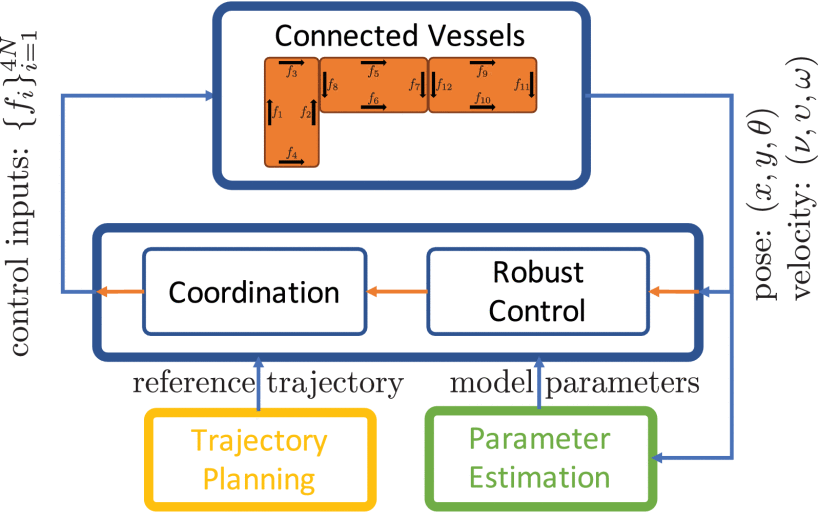
\includegraphics[width=0.6\textwidth]{park2019coordinatedSontrolScheme}
	\caption{Multi-vessel navigation system that consists of parameter estimation, trajectory planning, and coordinated robust control. \cite{park2019coordinated}. Note that the reference trajectory signal is not fed into the coordination block, although it might be interpreted as such on a first glance.}
	\label{fig:park2019coordinatedSontrolScheme}
\end{figure}